% Physics experiment report
% 1/Oct/2016

\documentclass[a4paper,10pt,notitlepage]{report}

\usepackage{CJKutf8}
\usepackage{amsmath}
\usepackage{indentfirst}
\usepackage{graphicx}

\setlength{\parindent}{2em} 

\begin{CJK*}{UTF8}{gbsn}
\begin{document}

\title{模拟示波器实验报告}
\author{秦光辉\ 9组3号}
\maketitle

\section*{一、实验数据处理}
\subsection*{1.周期,电压的测量}

	模拟示波器实验中我一共测了两组数据.第一组对应于500Hz,第二组对应于5kHz.表一是周期和频率实验数据,$\Delta t$为示波器每一格代表的时间长度,$t_L$是波形左侧峰值的读数,$ t_R $为右侧读书,而$T_1$是算出来的周期,$f$是利用周期算得的频率值,$f_o$是示波器读出的频率,$\Delta t'$是用示波器提供的光标读出的周期,$f'$是利用上一个数值得到的频率. \\
	
\begin{table}[htbp]
\centering
	\begin{tabular}{|c|c|c|c|c|c|c|c|c|}
	
		\hline
		\# & $\Delta t$ & $t_L$ & $ t_R $ & $T_1$ & $f$ & $f_o$ & $\Delta t'$ & $f'$ \\
		\hline
		1 & 2ms & -2.00 & 3.05 & 10.1ms & 99.0Hz & 99.013Hz & 10.12ms & 98.81Hz \\
		\hline
		2 & 50$\mu s$ & -2.78 & 1.20 & 199$\mu s$ & 5.03kHz & 5.02 & 200.5$\mu s$ & 4.99kHz \\
		\hline
		\multicolumn{9}{c}{\scriptsize Table 1\ 示波器周期与频率实验数据表} \\

	\end{tabular}
\end{table}

	表二是电压测量数据.表中$K$是偏转因数,$U_u$是波形峰值在顶端的读书,$U_d$是底端的读数,$U_{pp}$是电压的峰峰值数据,$U_e$是利用峰峰值电压测得的有效值电压,$\delta V$是用示波器的光标读得的电压值. \\

\begin{table}[htbp]
\centering
	\begin{tabular}{|c|c|c|c|c|c|c|}
	
		\hline
		\# & $K$ & $U_u$ & $U_d$ & $U_{pp}$ & $U_e$ & $\delta V$  \\
		\hline
		1 & 5V & 2.00 & -2.28 & 21.4V & 7.57V & 21.65V \\
		\hline
		2 & 5V & 2.00 & -2.27 & 21.4V & 7.57V & 21.60V \\
		\hline
		\multicolumn{7}{c}{\scriptsize Table 2\ 示波器电压实验数据表} \\

	\end{tabular}
\end{table}

\subsection*{2.利萨如图形观察}
	
	我利用两个信号发生器,获得了一些利萨如图形,如图1-10所示.	\\
	\\
	\\
	\\
	
\begin{figure}[htbp]
\centering

	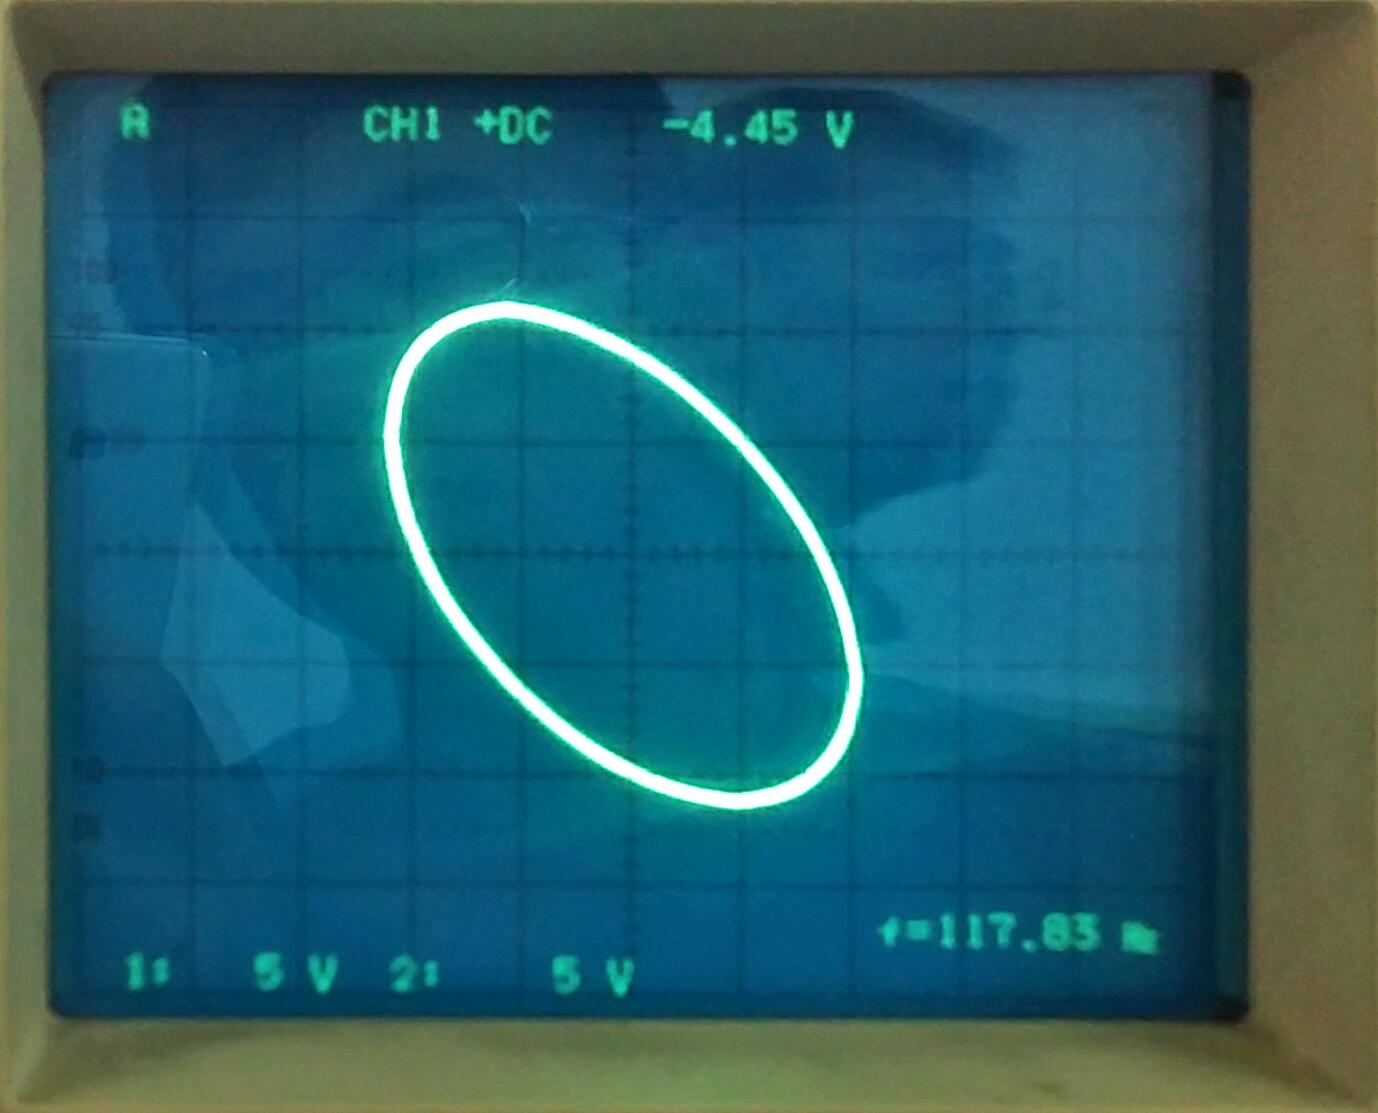
\includegraphics[scale=.2]{L01.jpg}
	\begin{center}
		\scriptsize Figure 1 利萨如图形1
	\end{center}

\end{figure}
	
\begin{figure}[htbp]
\centering

	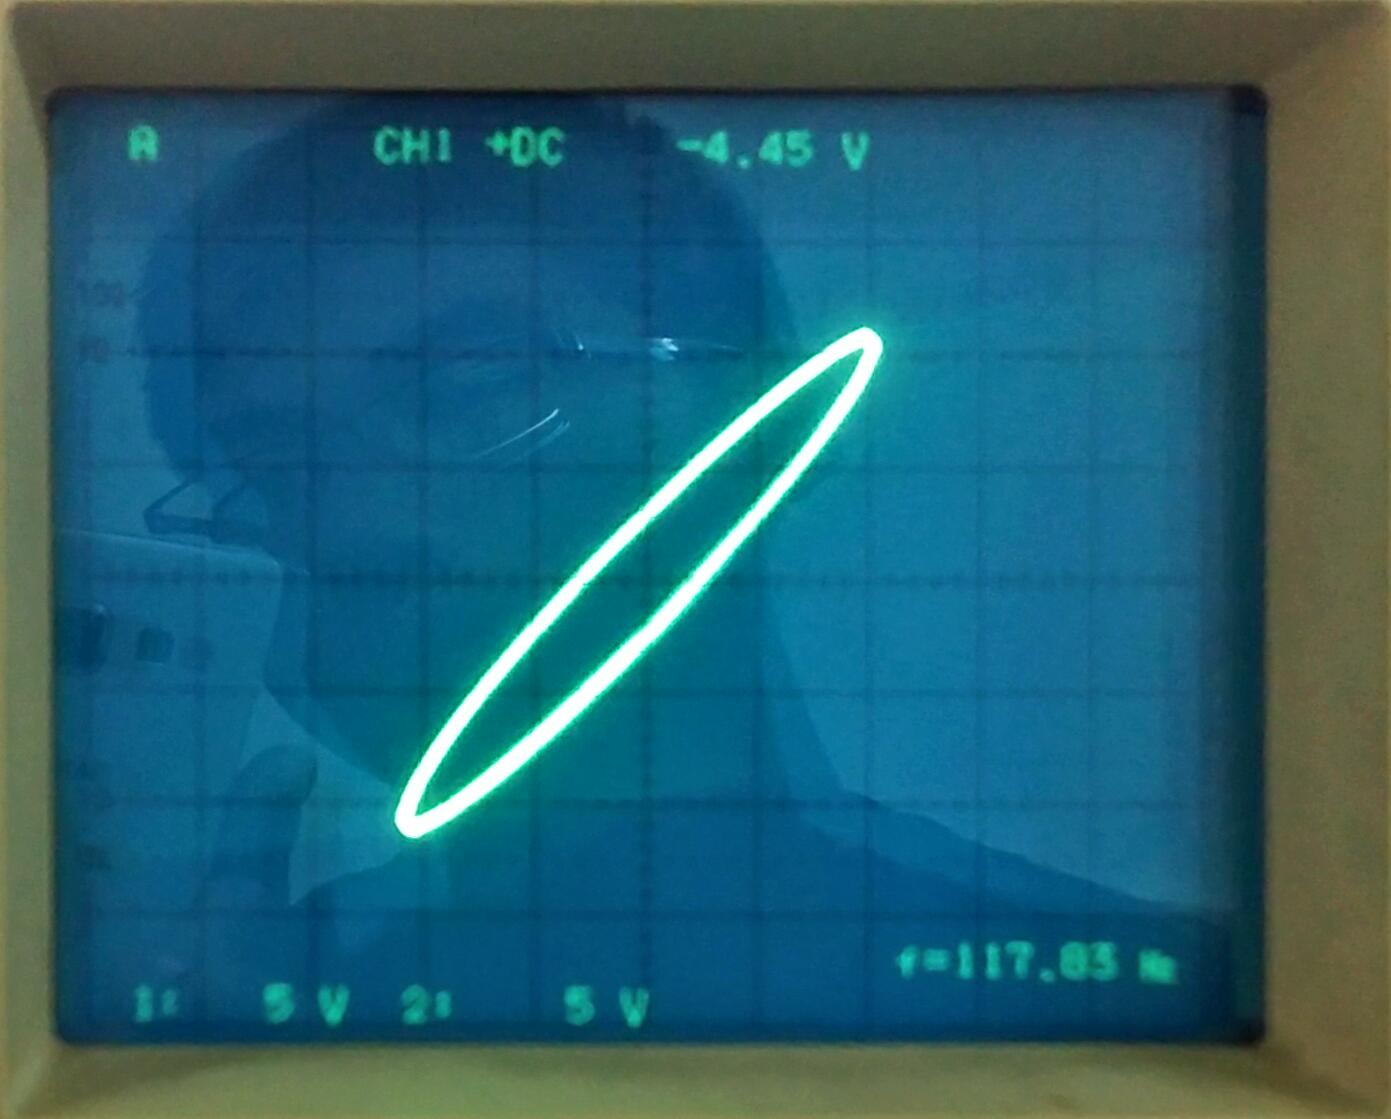
\includegraphics[scale=.2]{L02.jpg}
	\begin{center}
		\scriptsize Figure 2 利萨如图形2
	\end{center}

\end{figure}
	
\begin{figure}[htbp]
\centering

	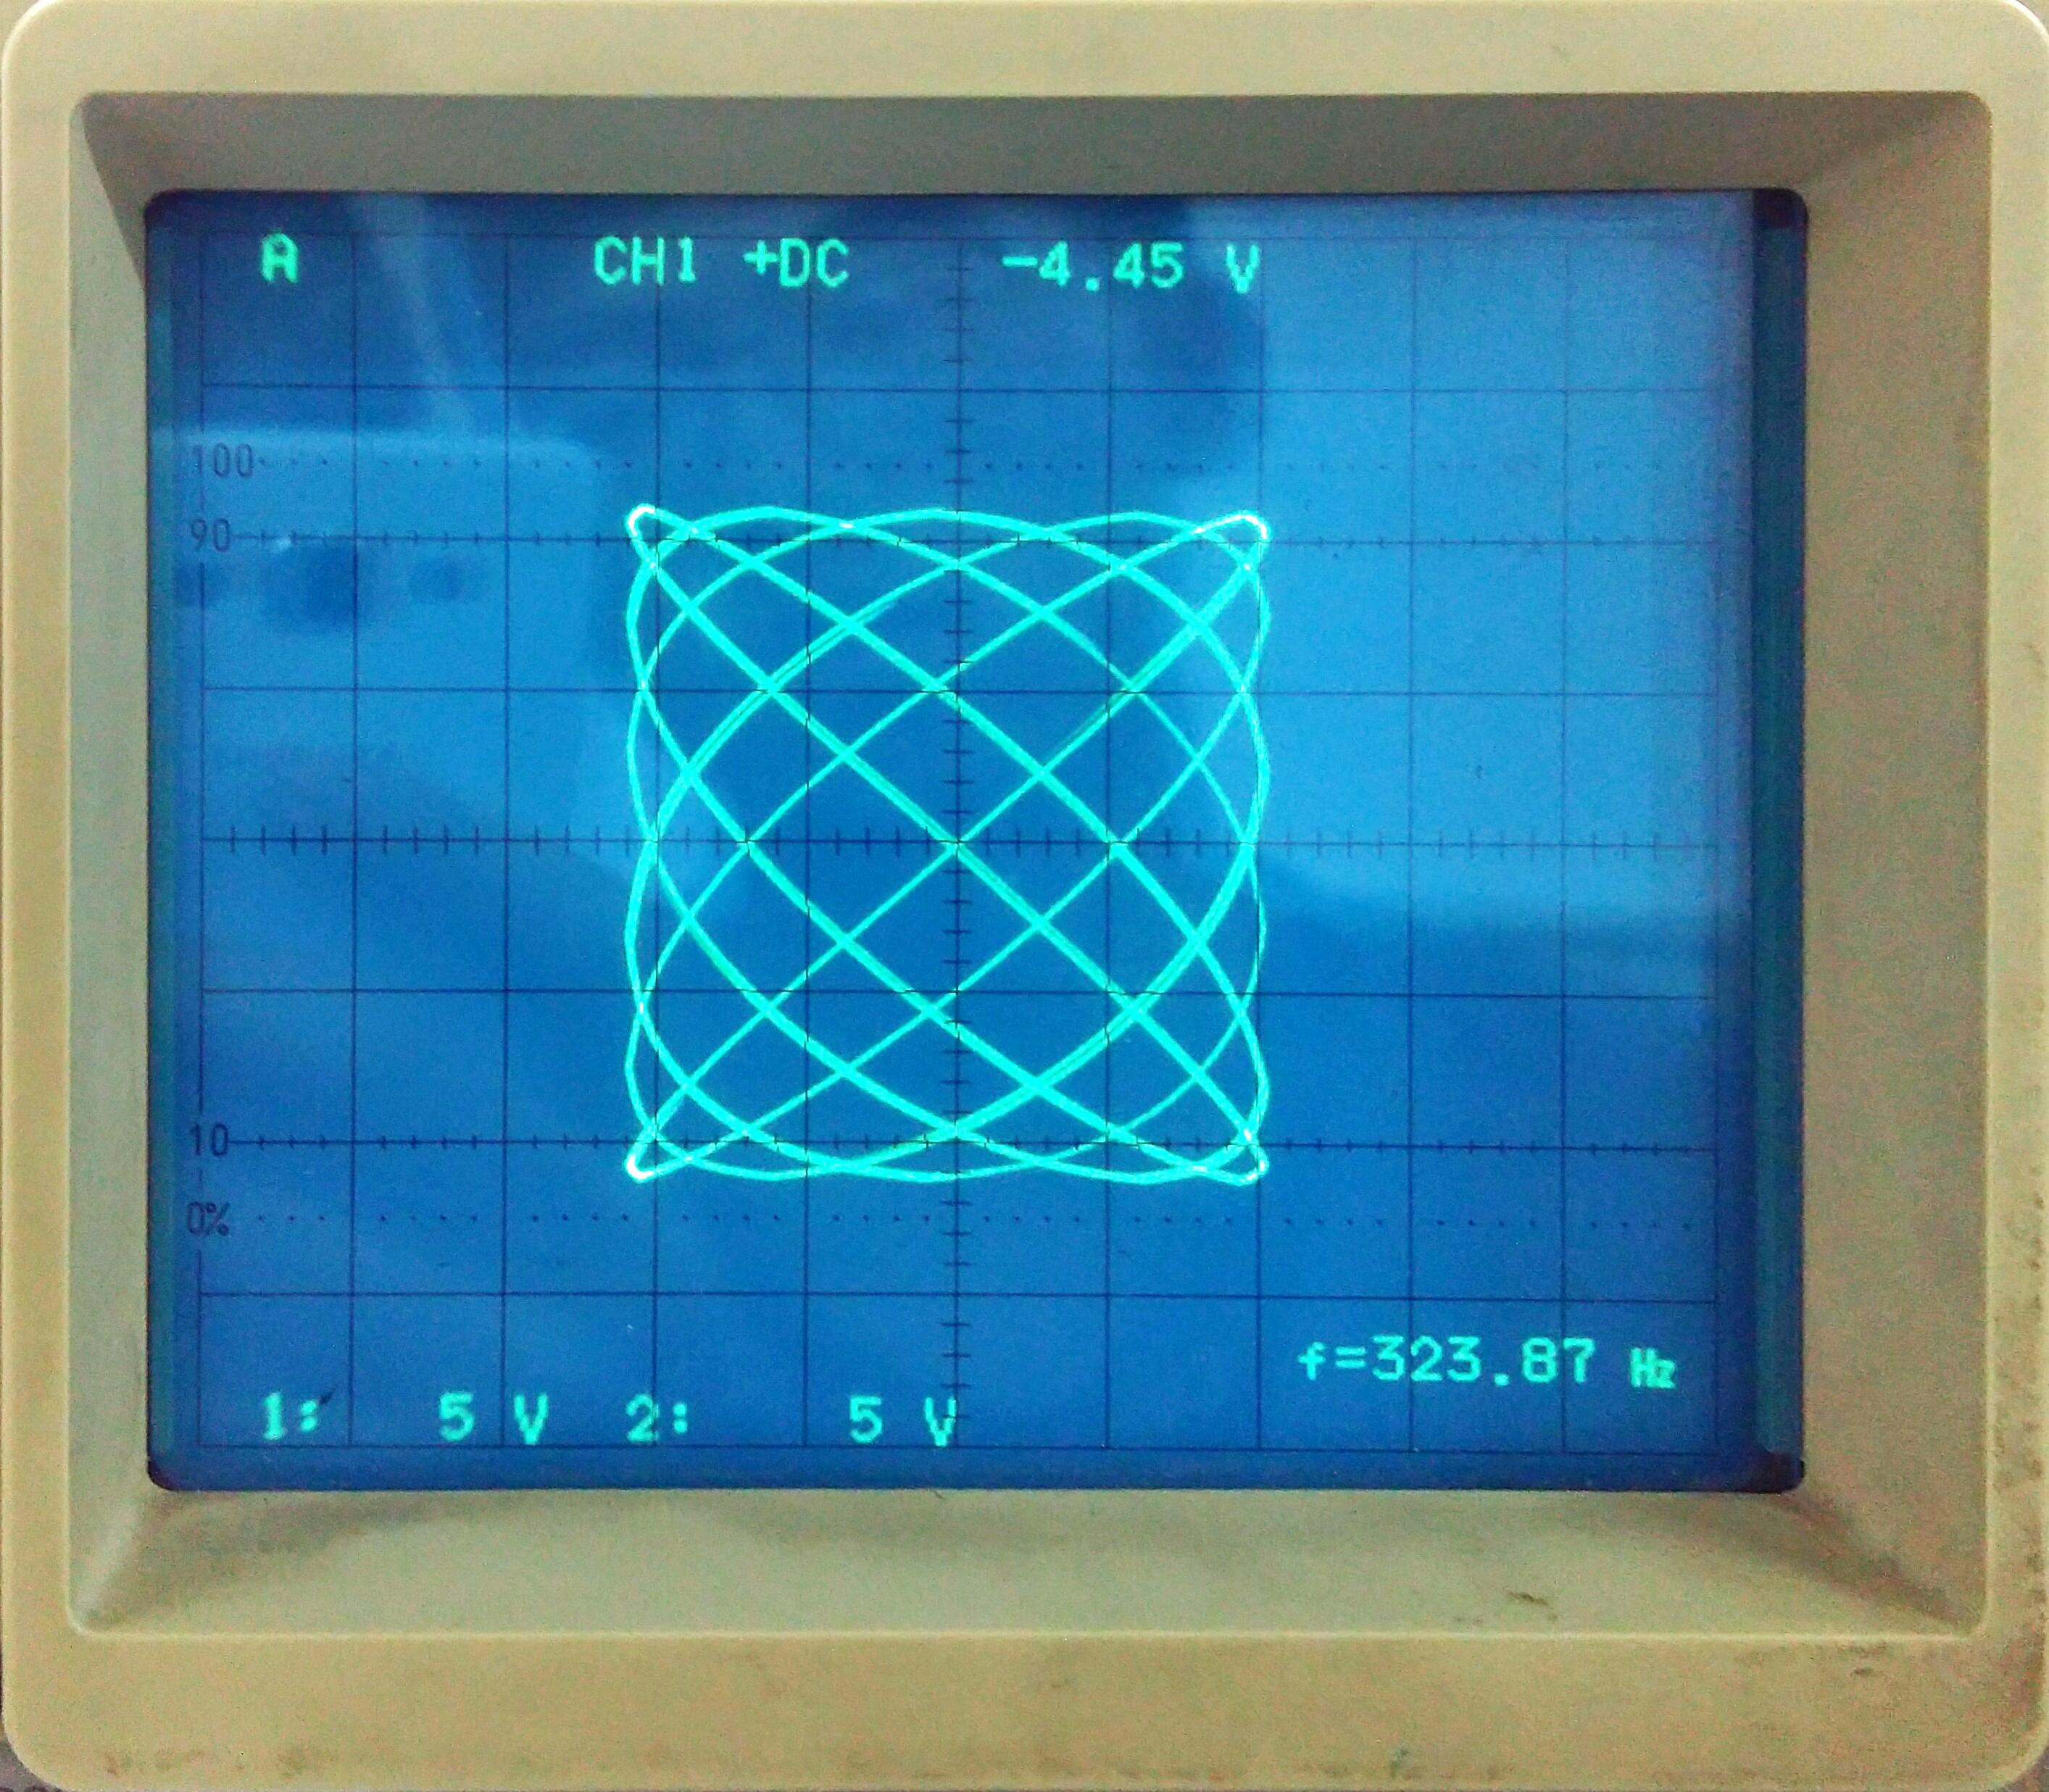
\includegraphics[scale=.1]{L03.jpg}
	\begin{center}
		\scriptsize Figure 3 利萨如图形3
	\end{center}

\end{figure}
	
\begin{figure}[htbp]
\centering

	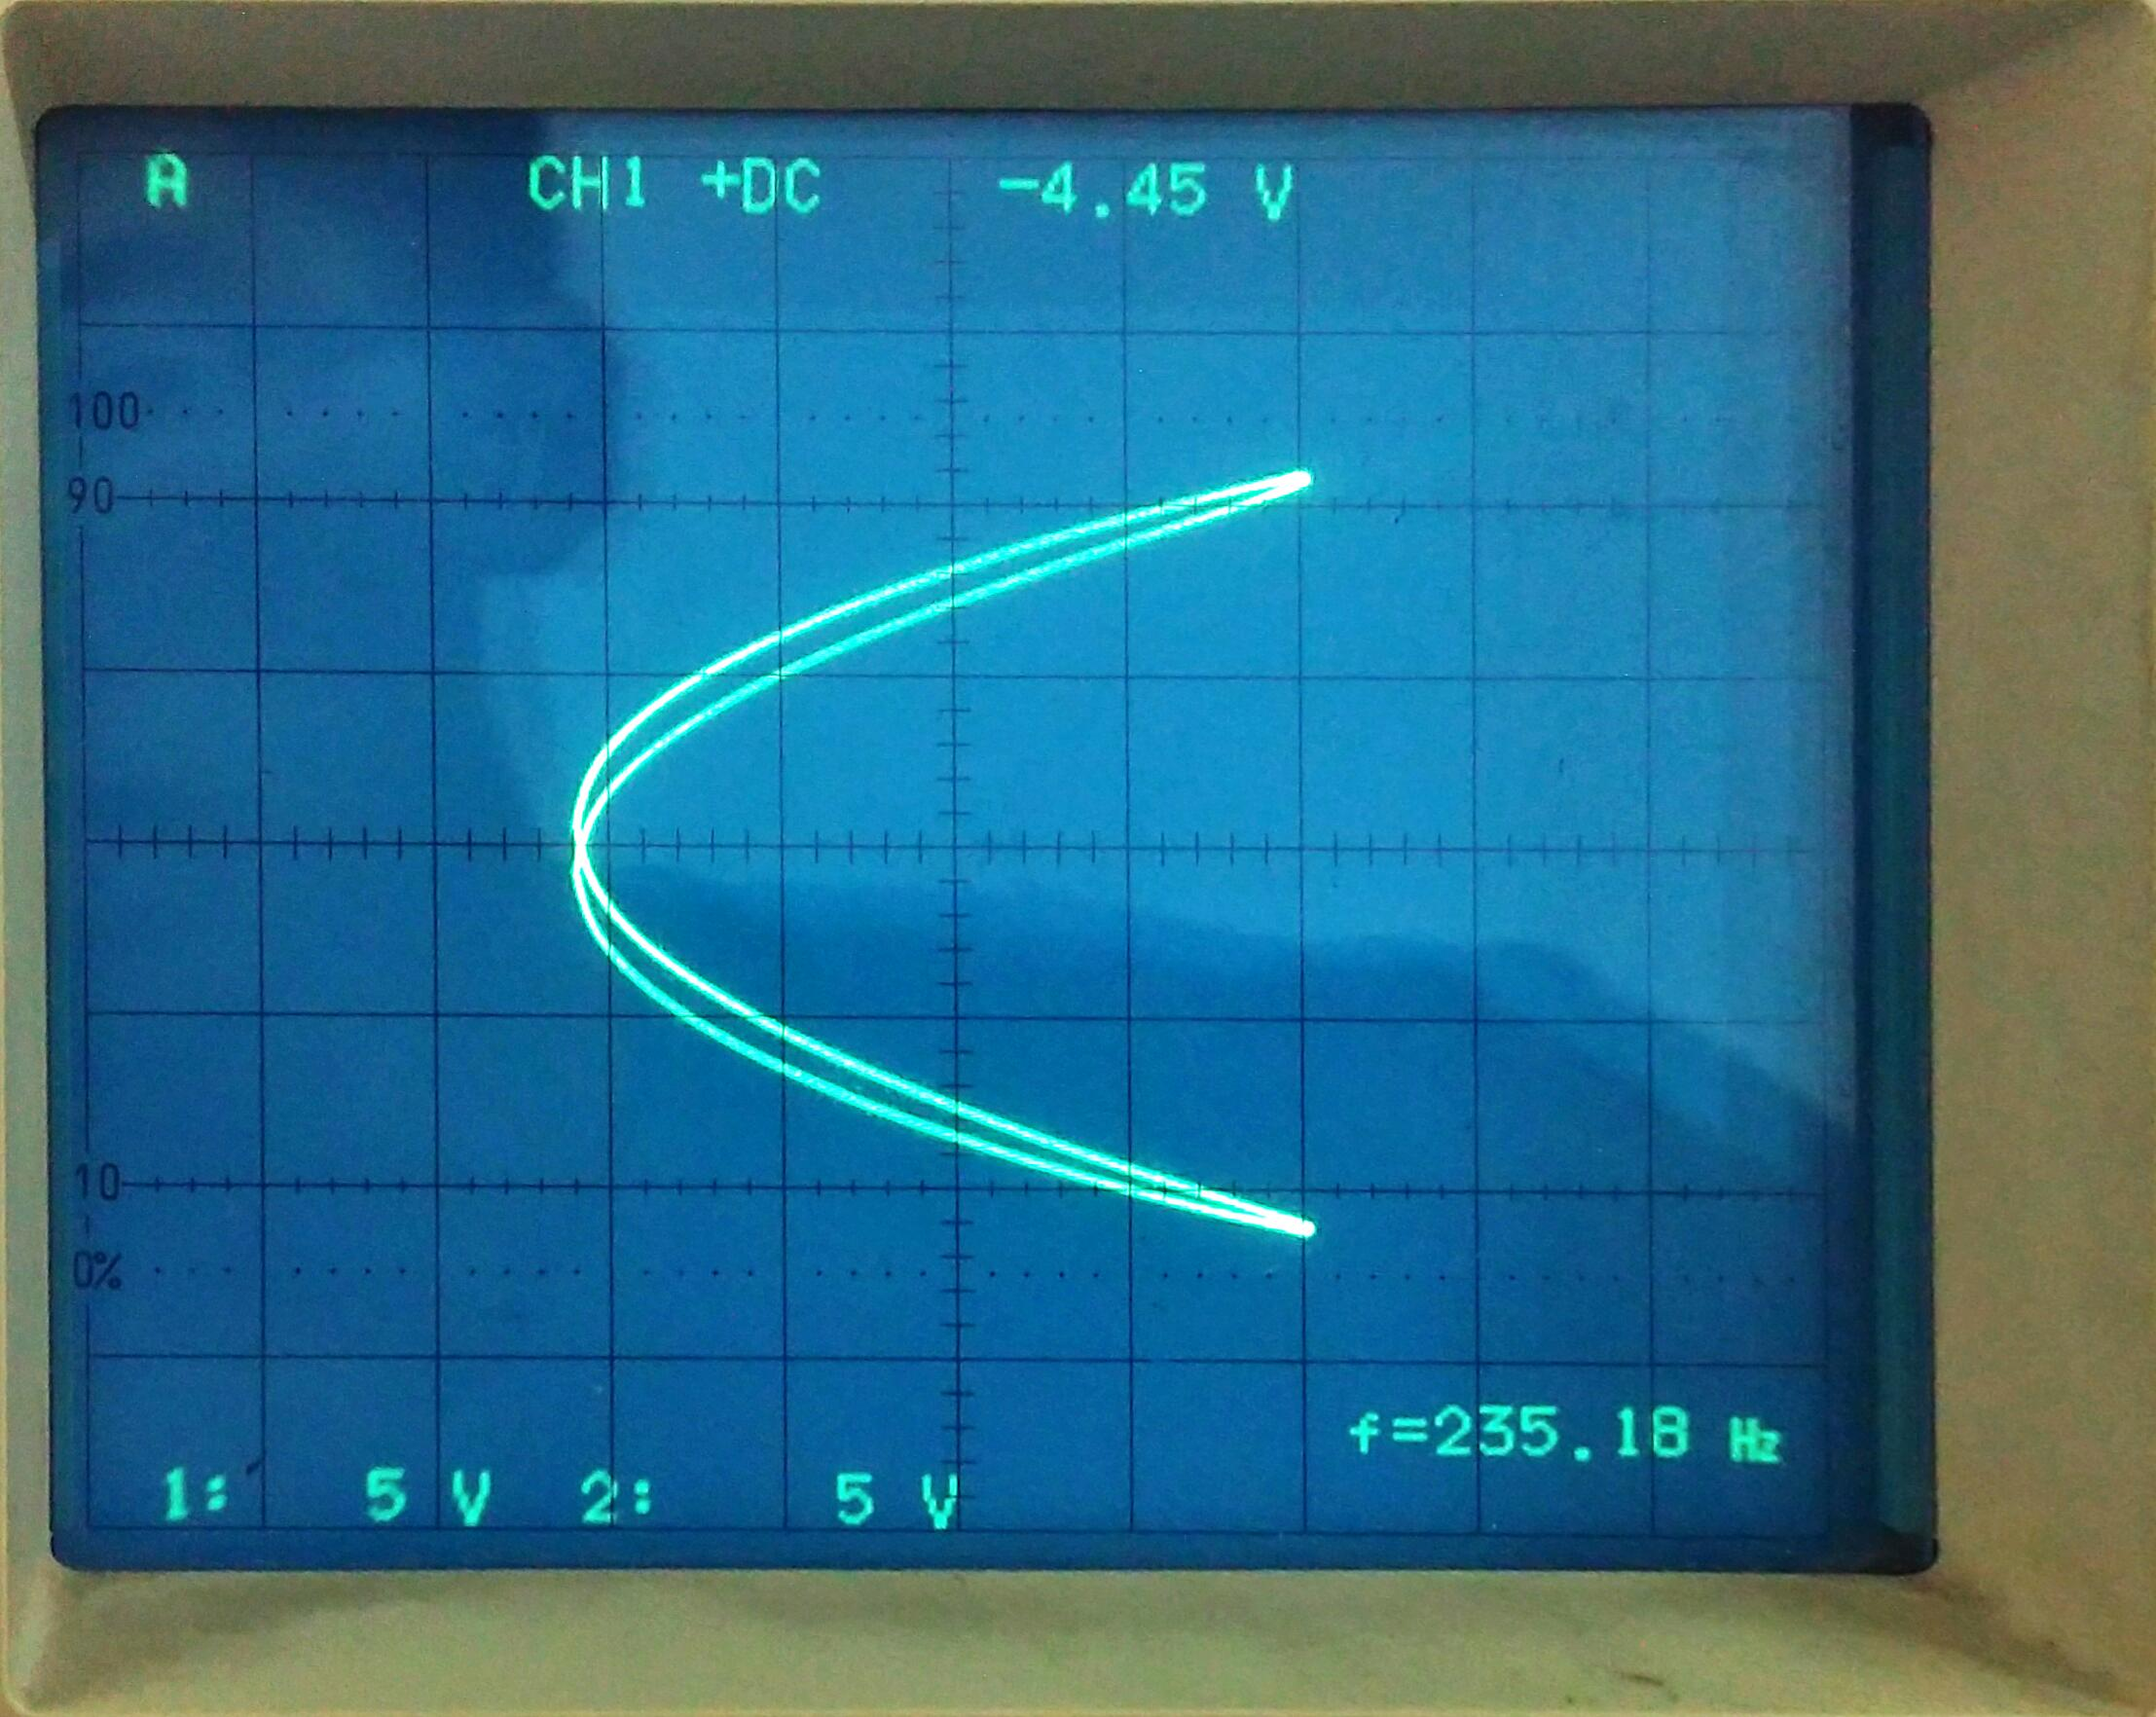
\includegraphics[scale=.13]{L04.jpg}
	\begin{center}
		\scriptsize Figure 4 利萨如图形4
	\end{center}

\end{figure}
	
\begin{figure}[htbp]
\centering

	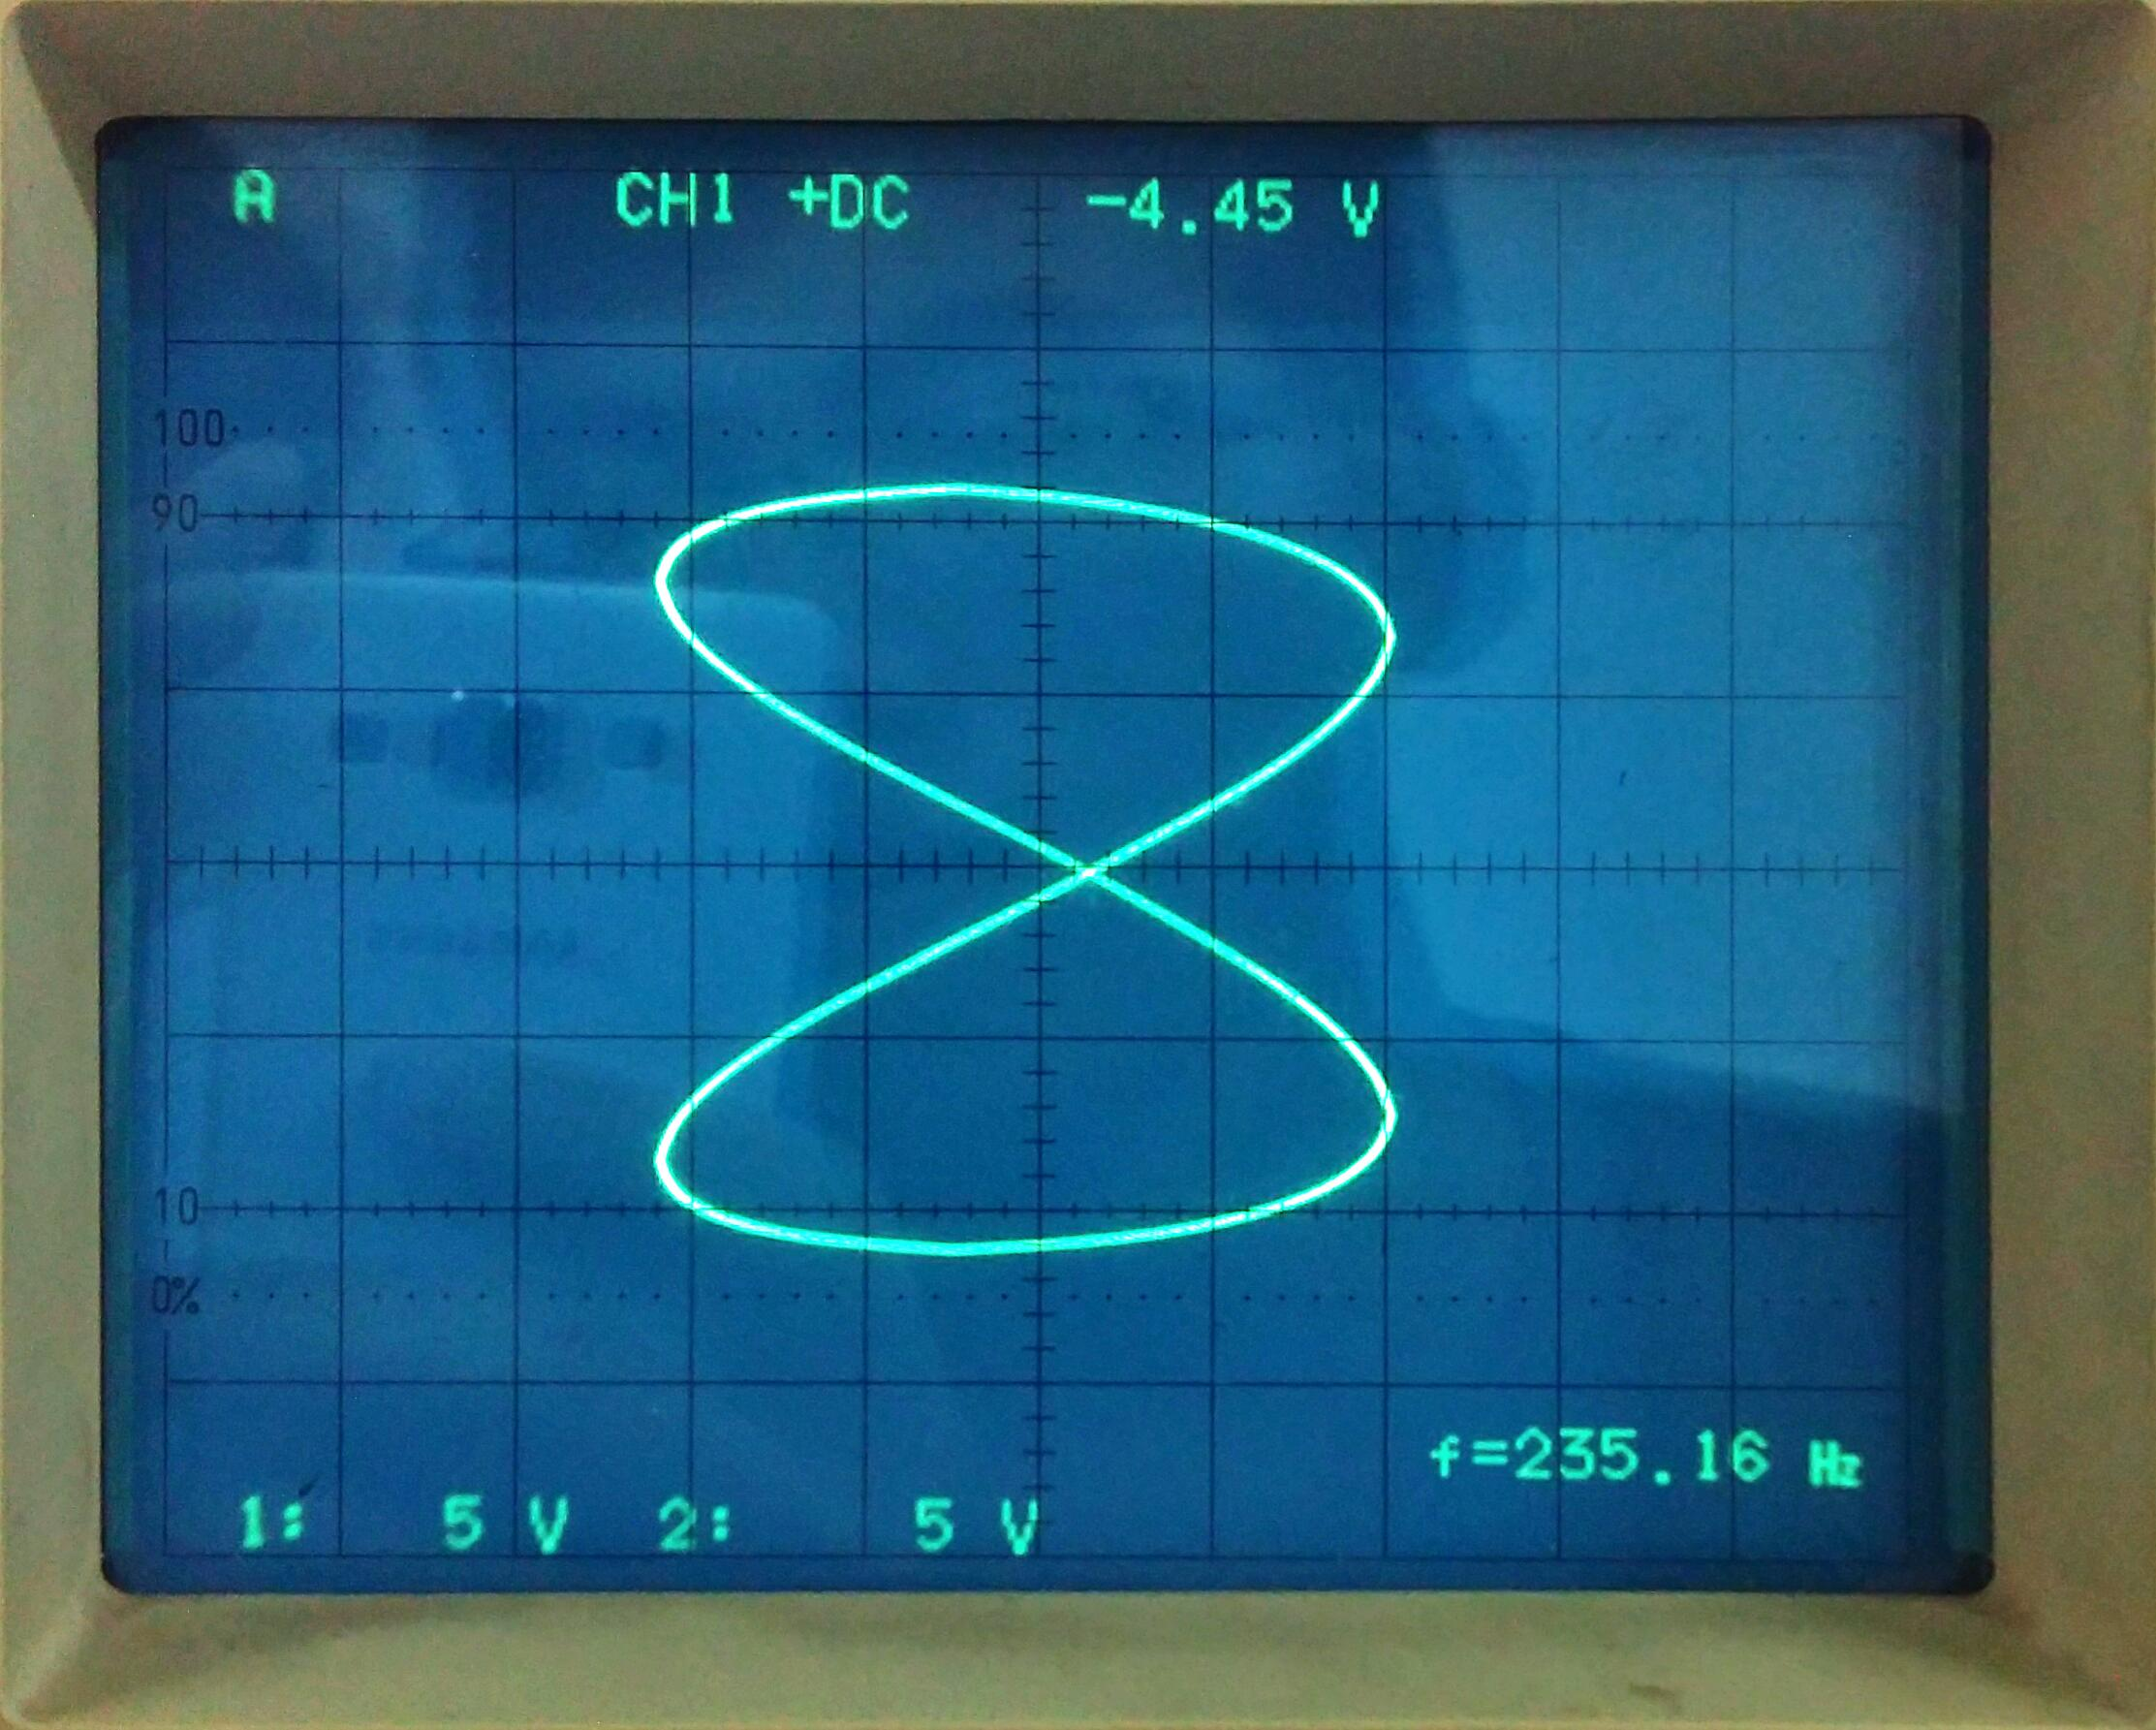
\includegraphics[scale=.13]{L05.jpg}
	\begin{center}
		\scriptsize Figure 5 利萨如图形5
	\end{center}

\end{figure}
	
\begin{figure}[htbp]
\centering

	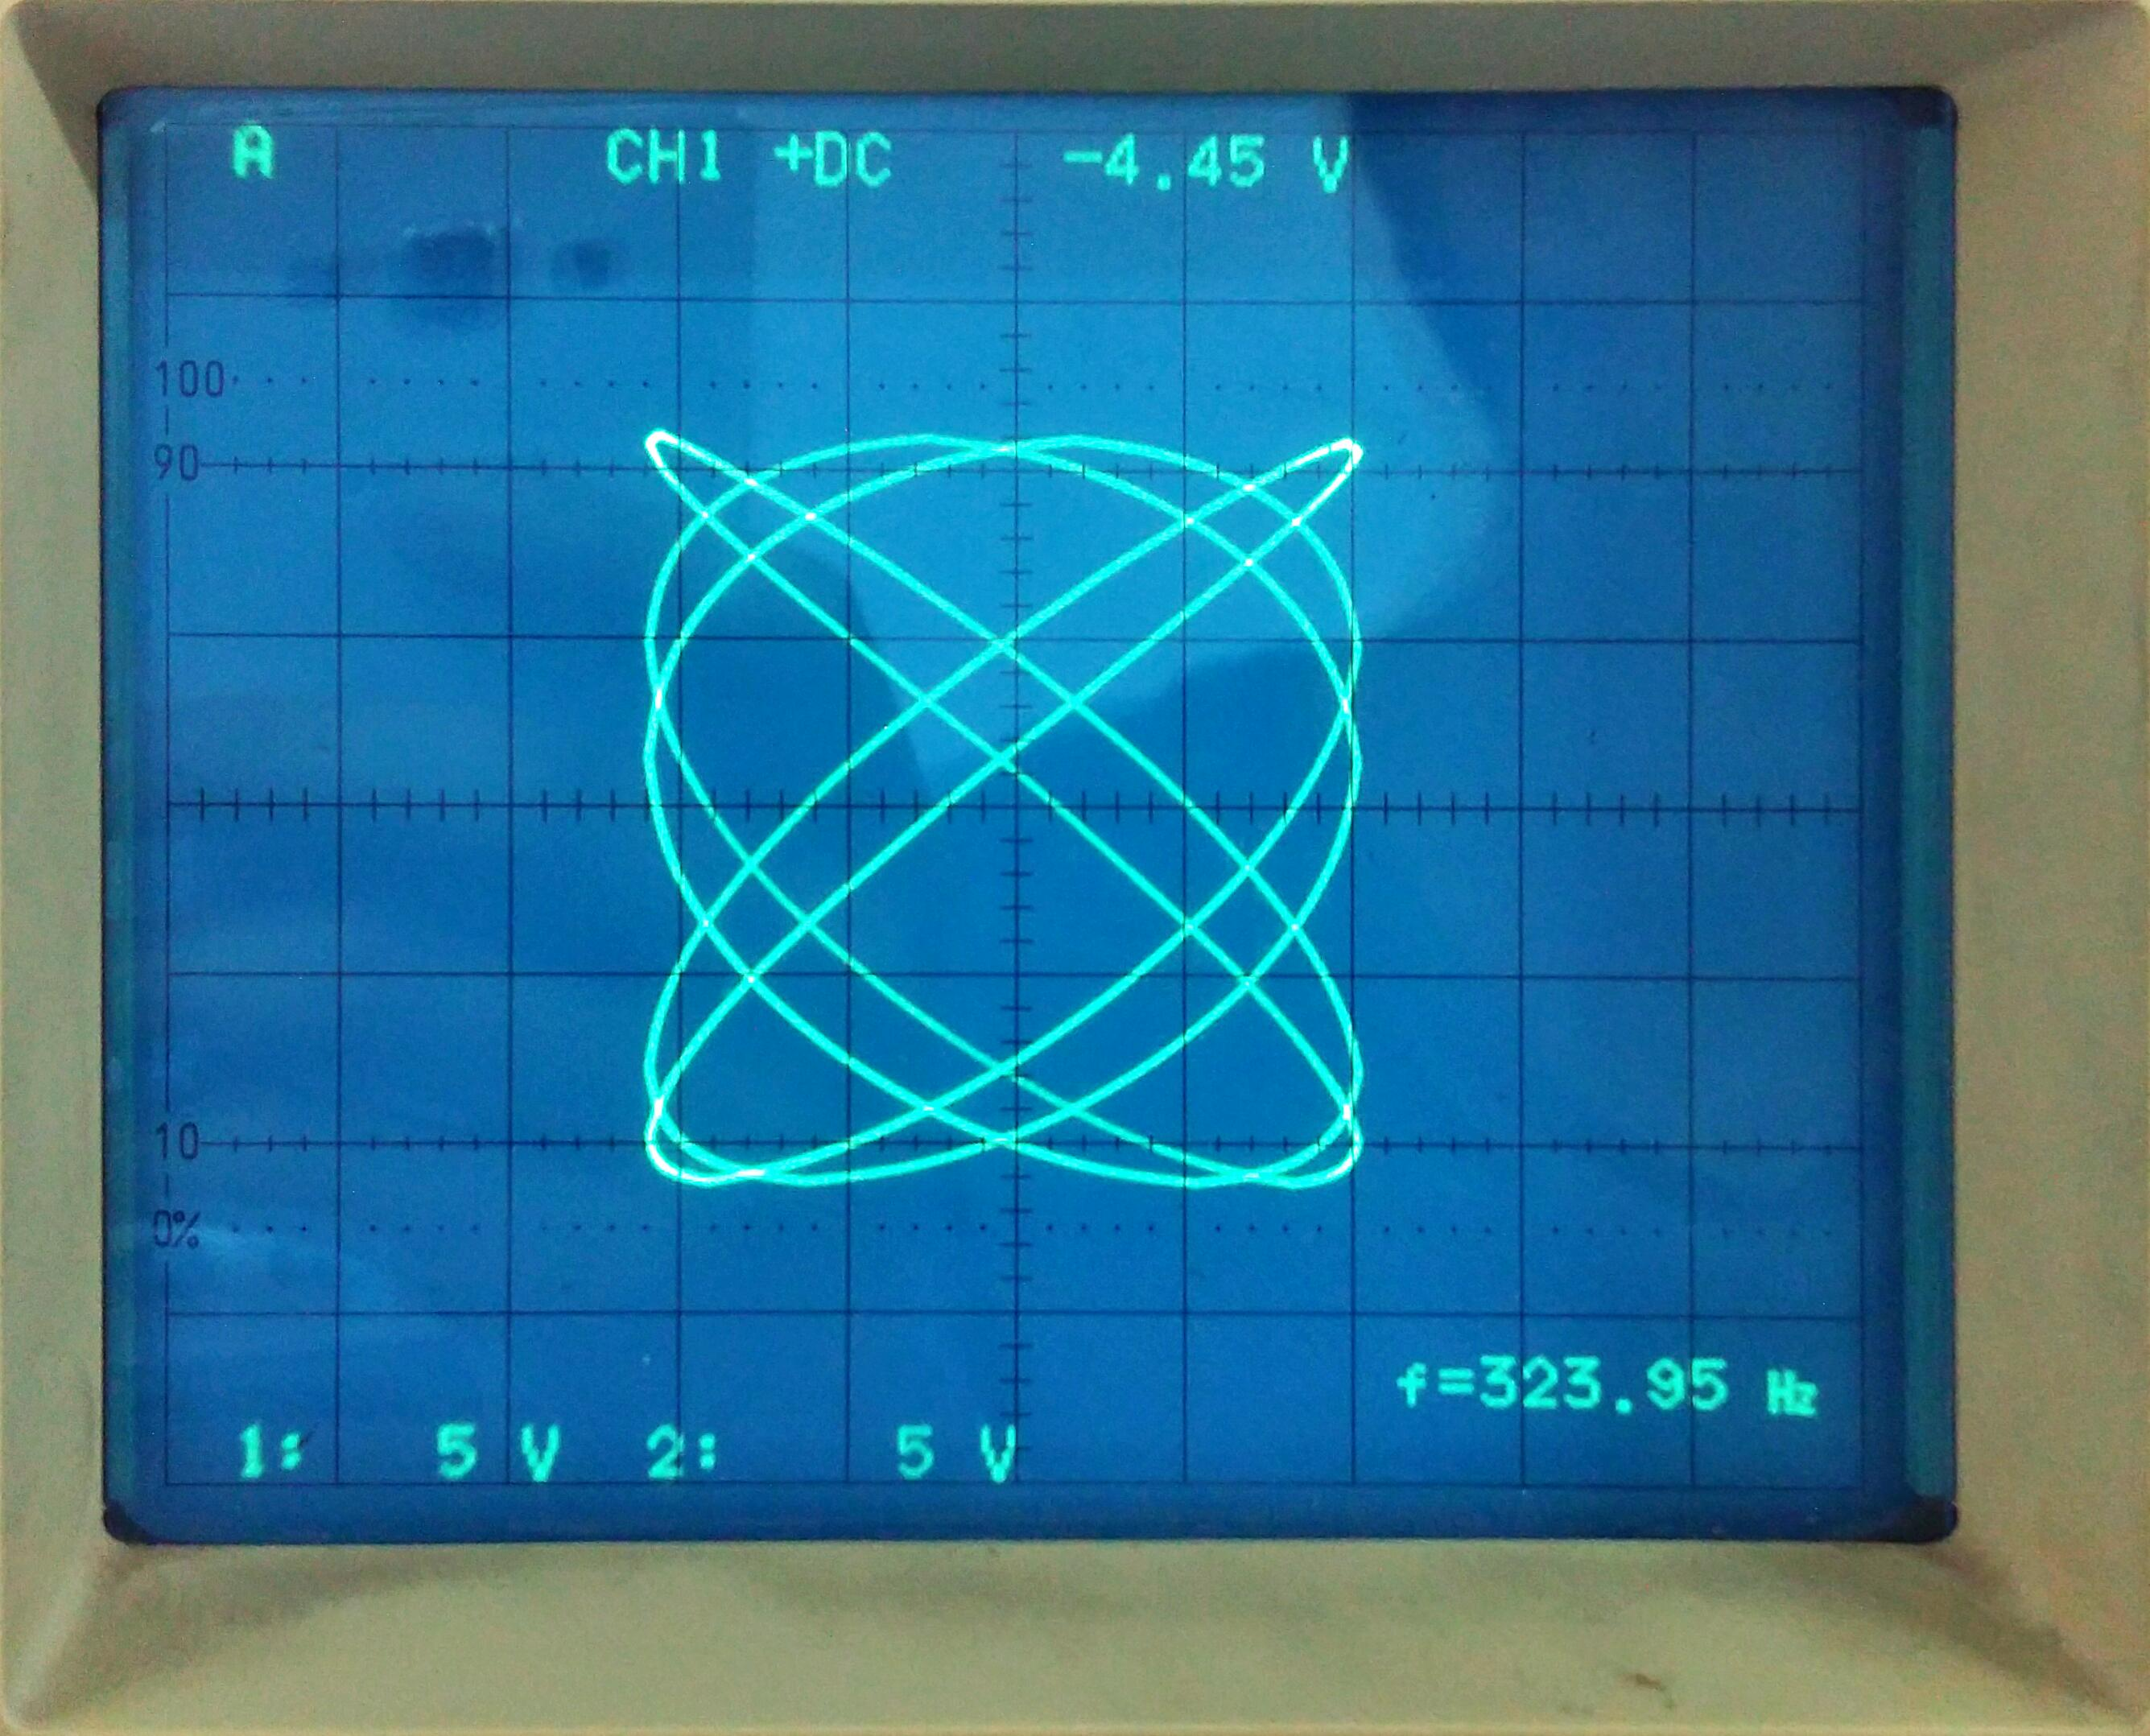
\includegraphics[scale=.1]{L06.jpg}
	\begin{center}
		\scriptsize Figure 6 利萨如图形6
	\end{center}

\end{figure}
	
\begin{figure}[htbp]
\centering

	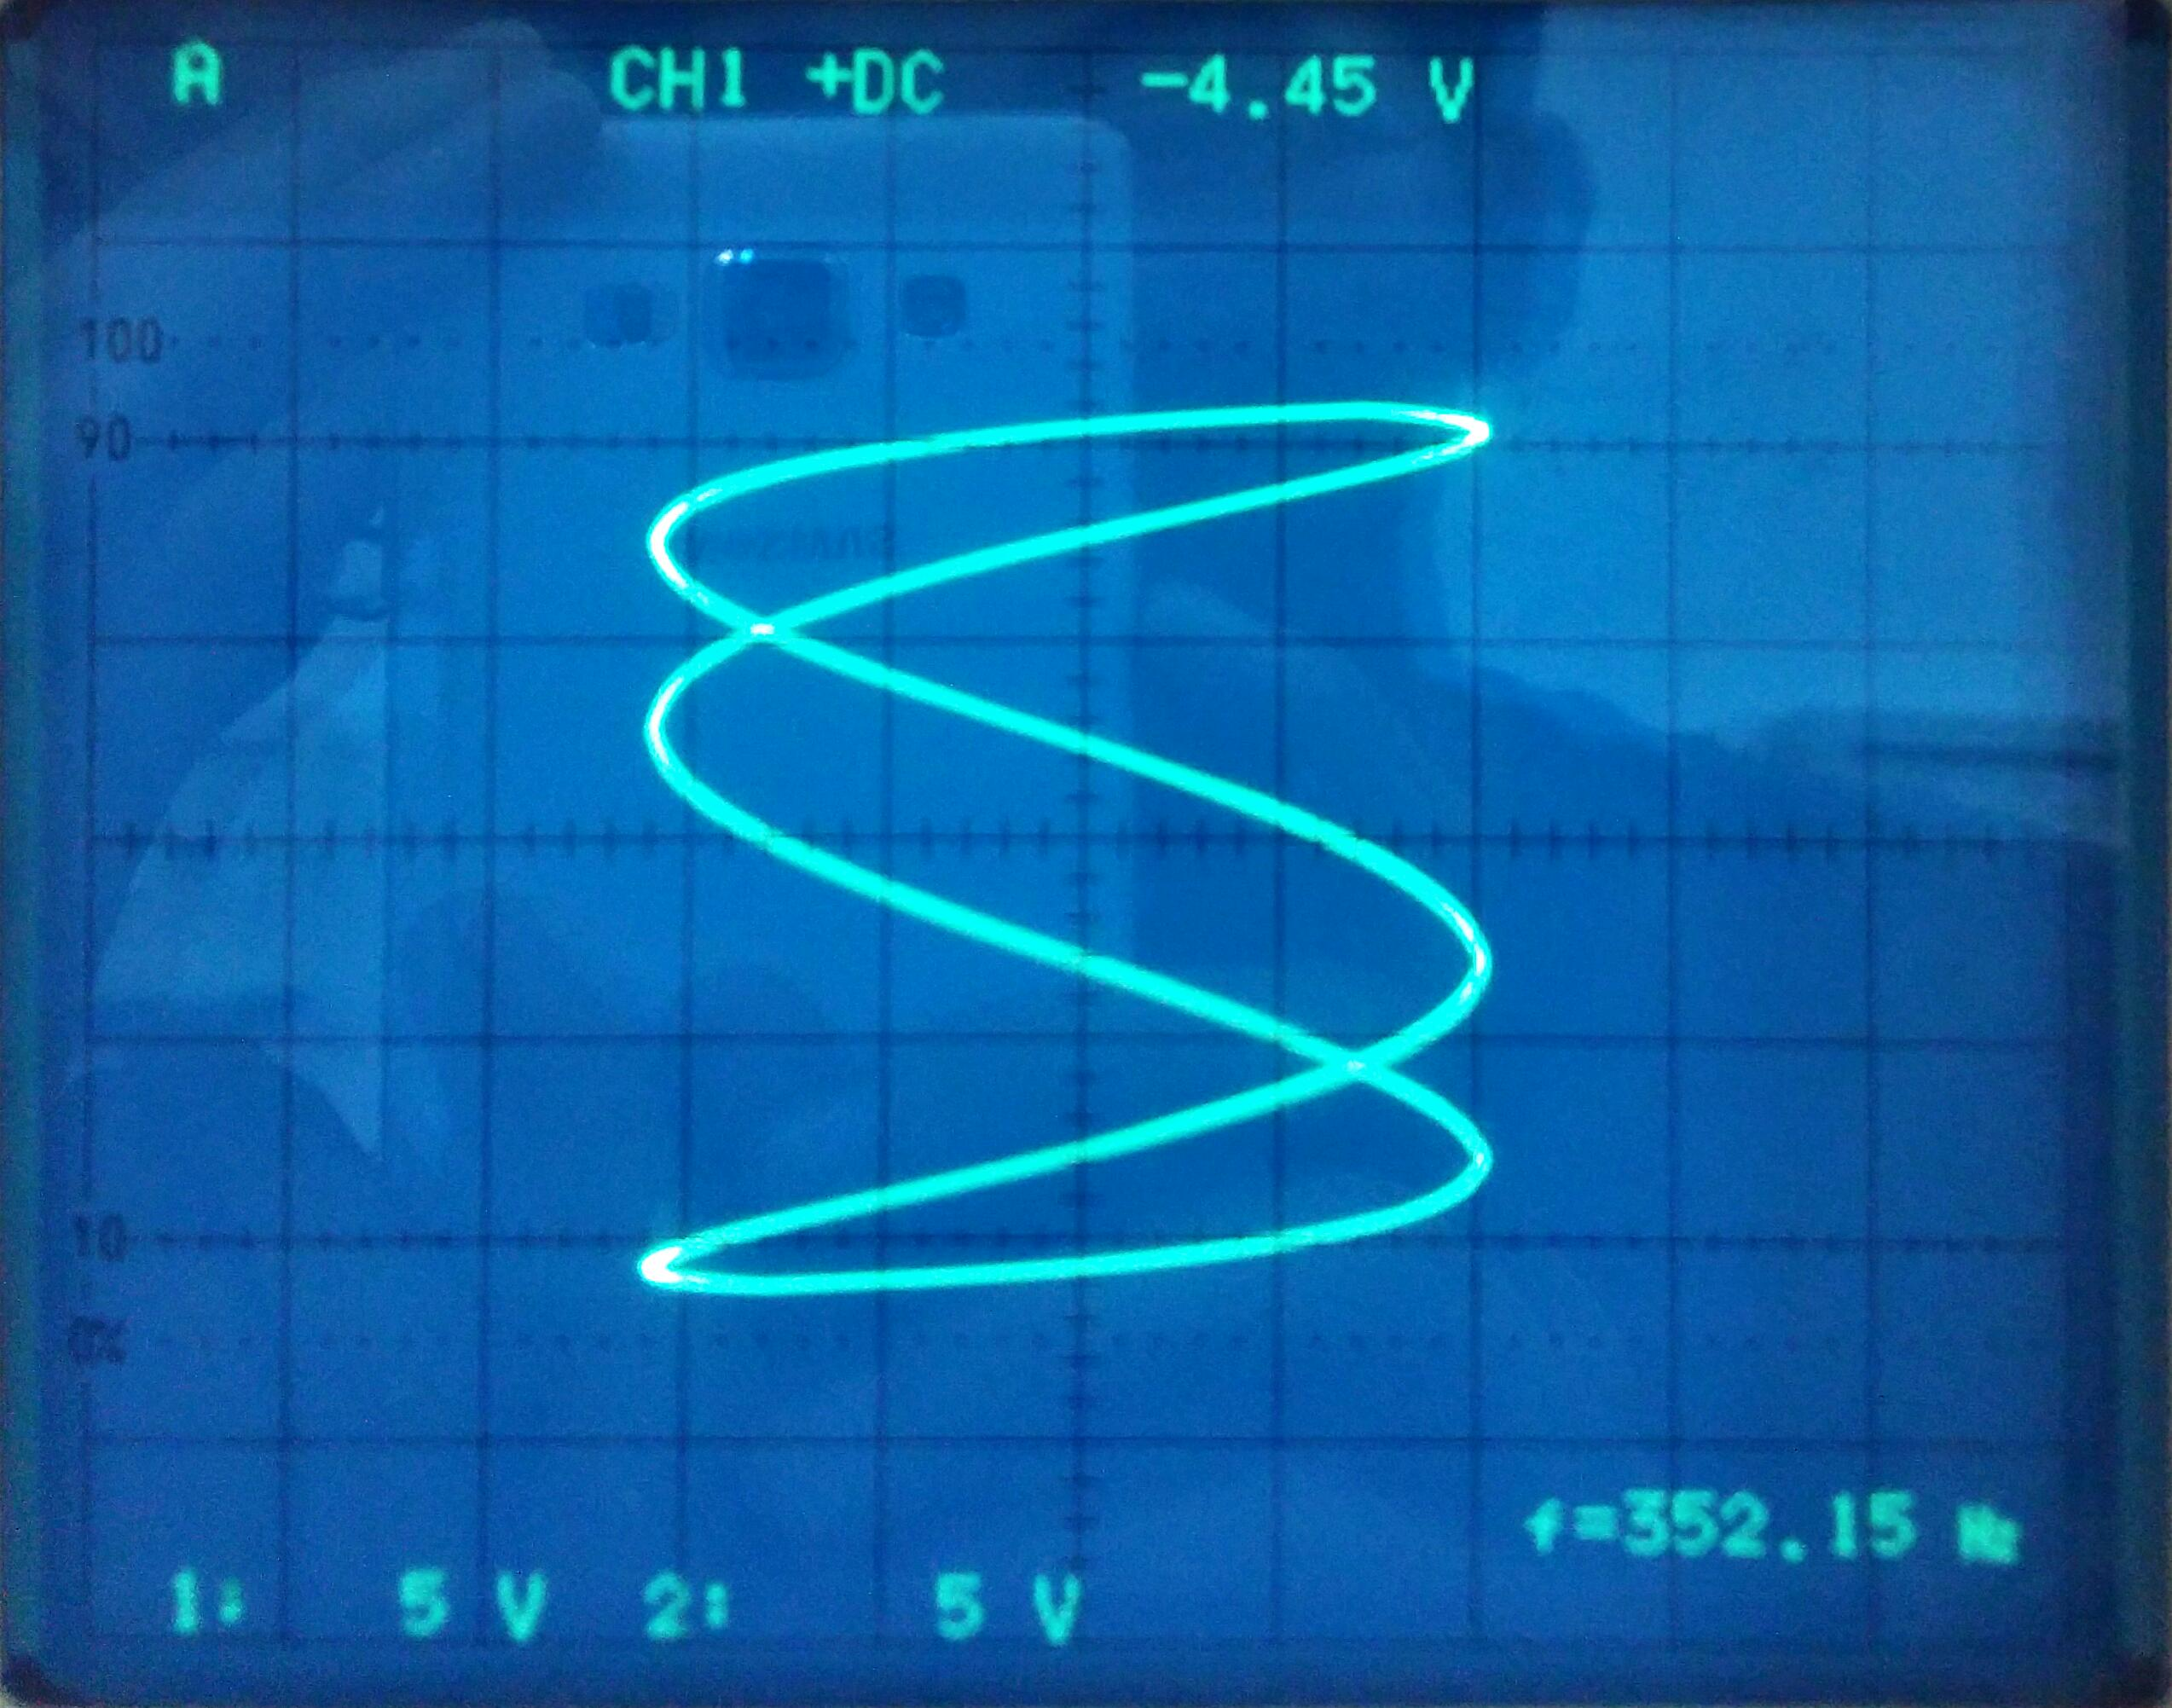
\includegraphics[scale=.1]{L07.jpg}
	\begin{center}
		\scriptsize Figure 7 利萨如图形7
	\end{center}

\end{figure}
	
\begin{figure}[htbp]
\centering

	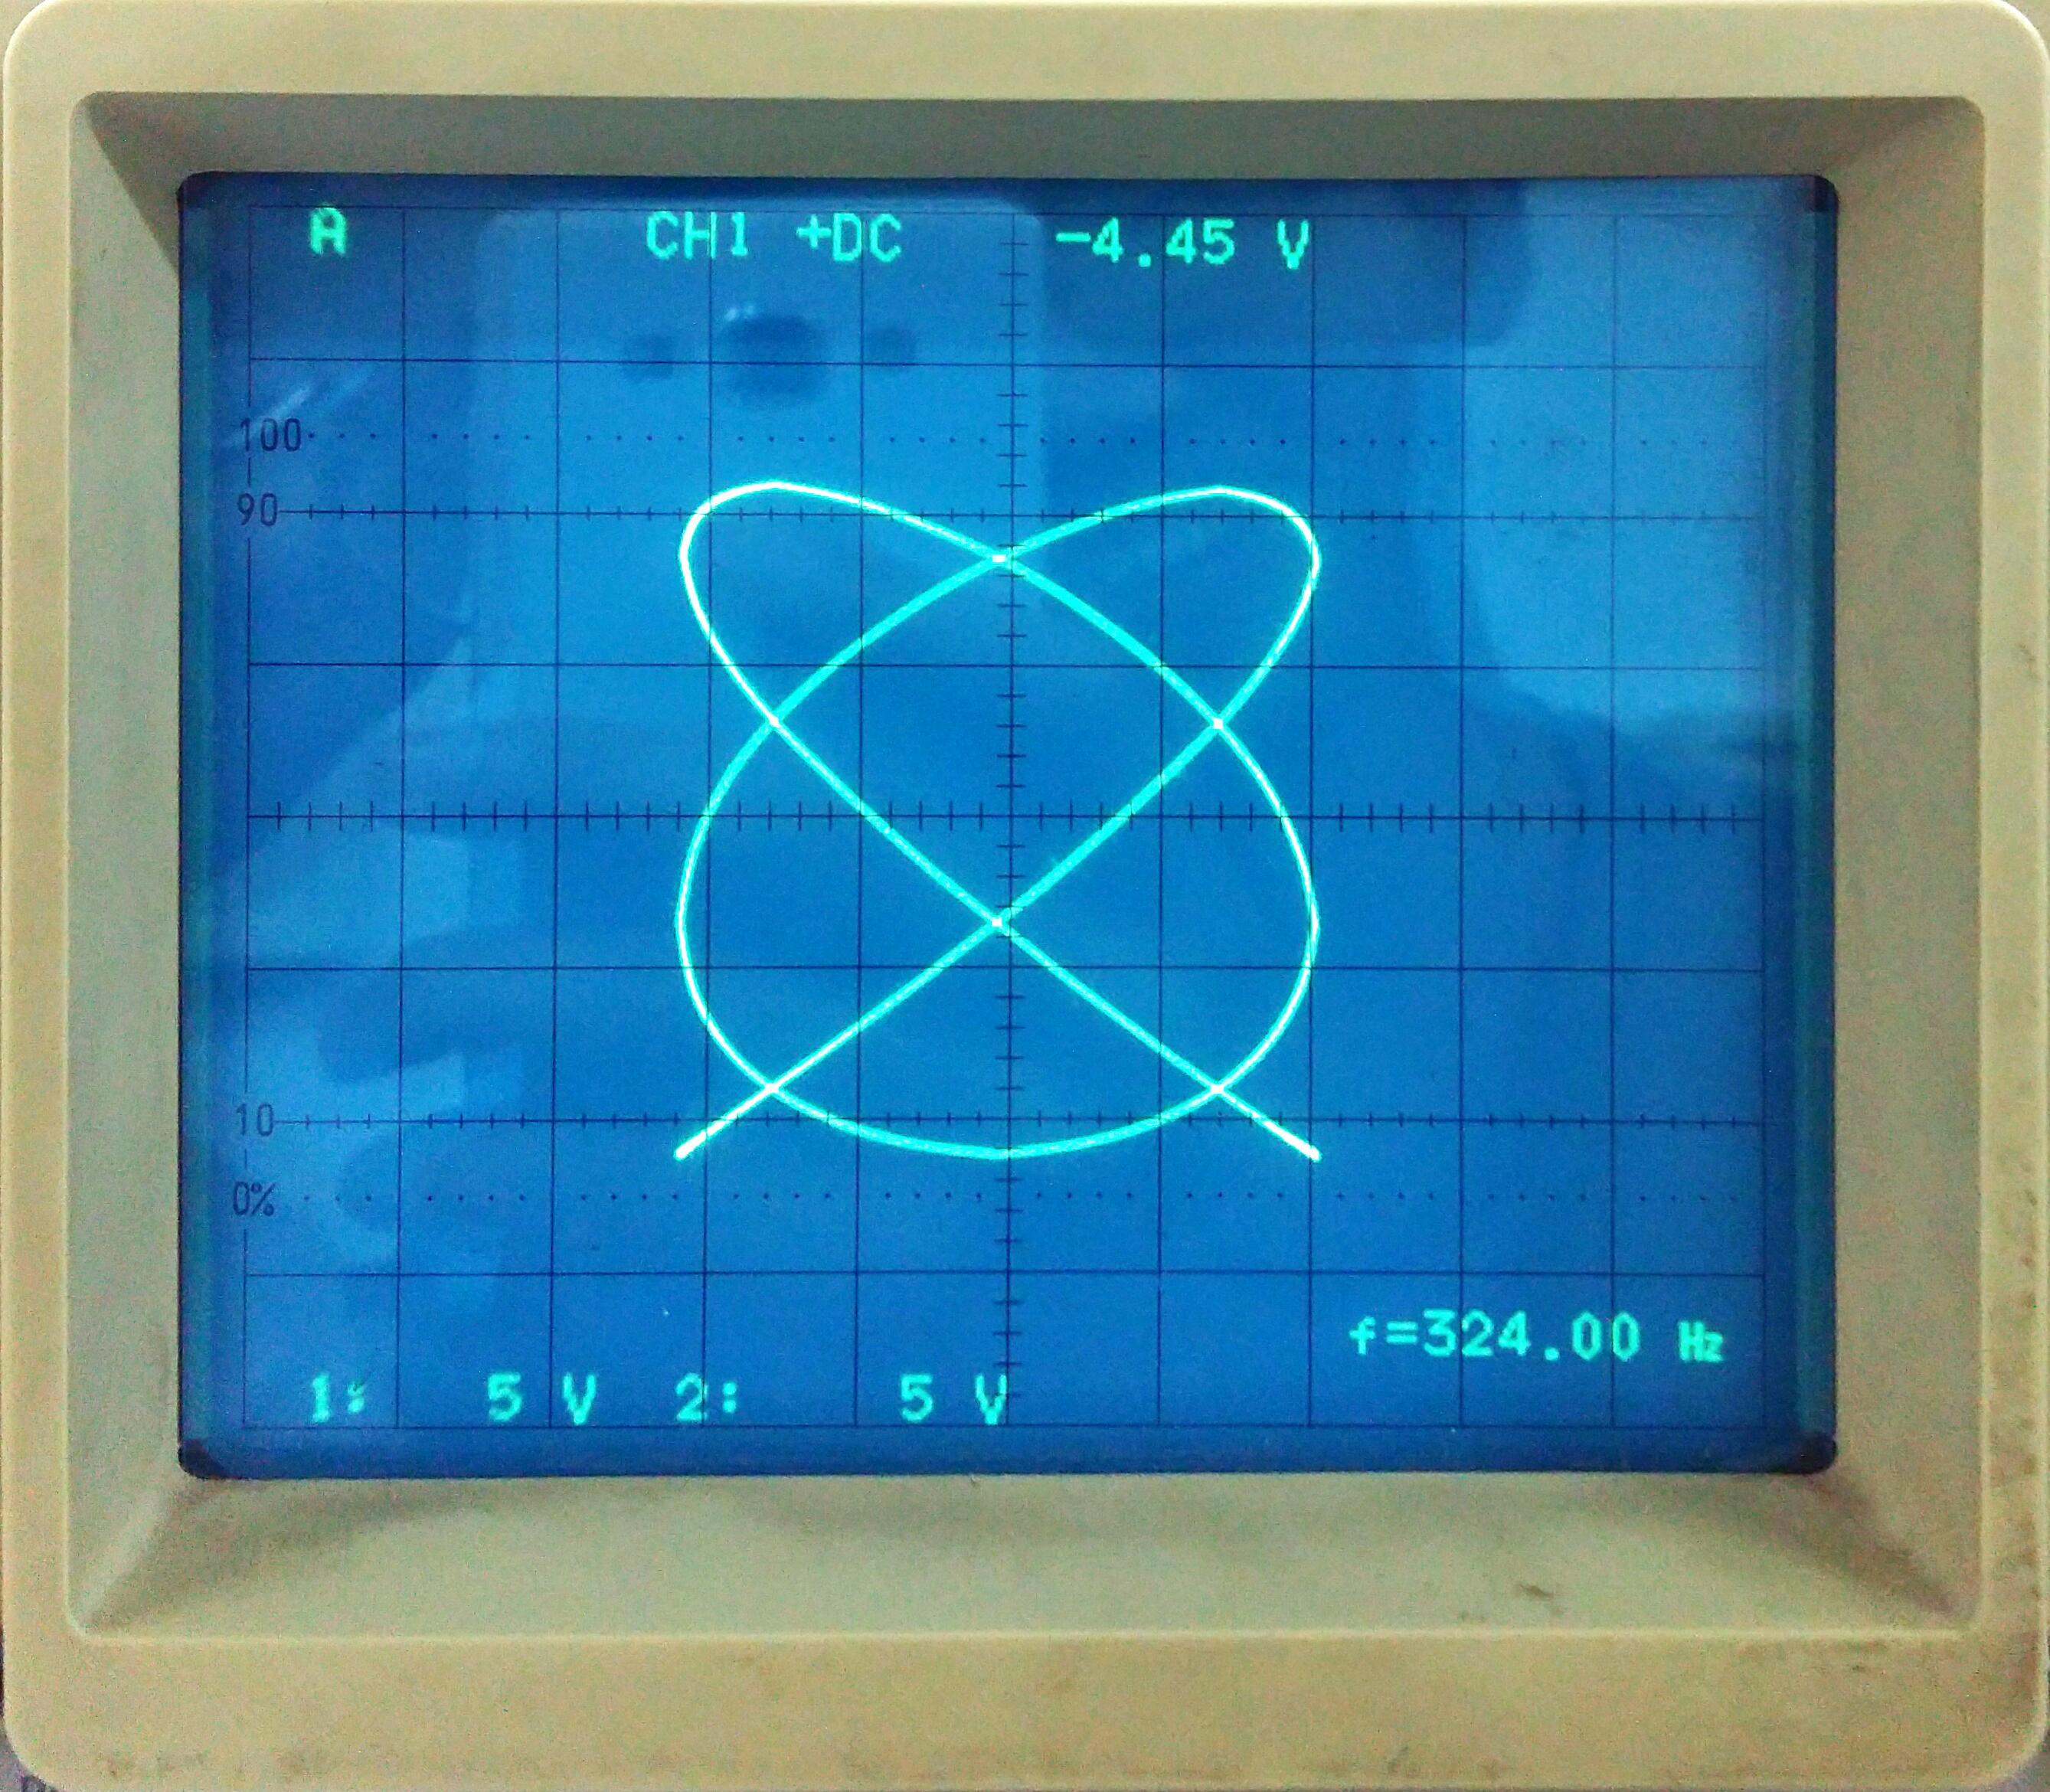
\includegraphics[scale=.1]{L08.jpg}
	\begin{center}
		\scriptsize Figure 8 利萨如图形8
	\end{center}

\end{figure}
	
\begin{figure}[htbp]
\centering

	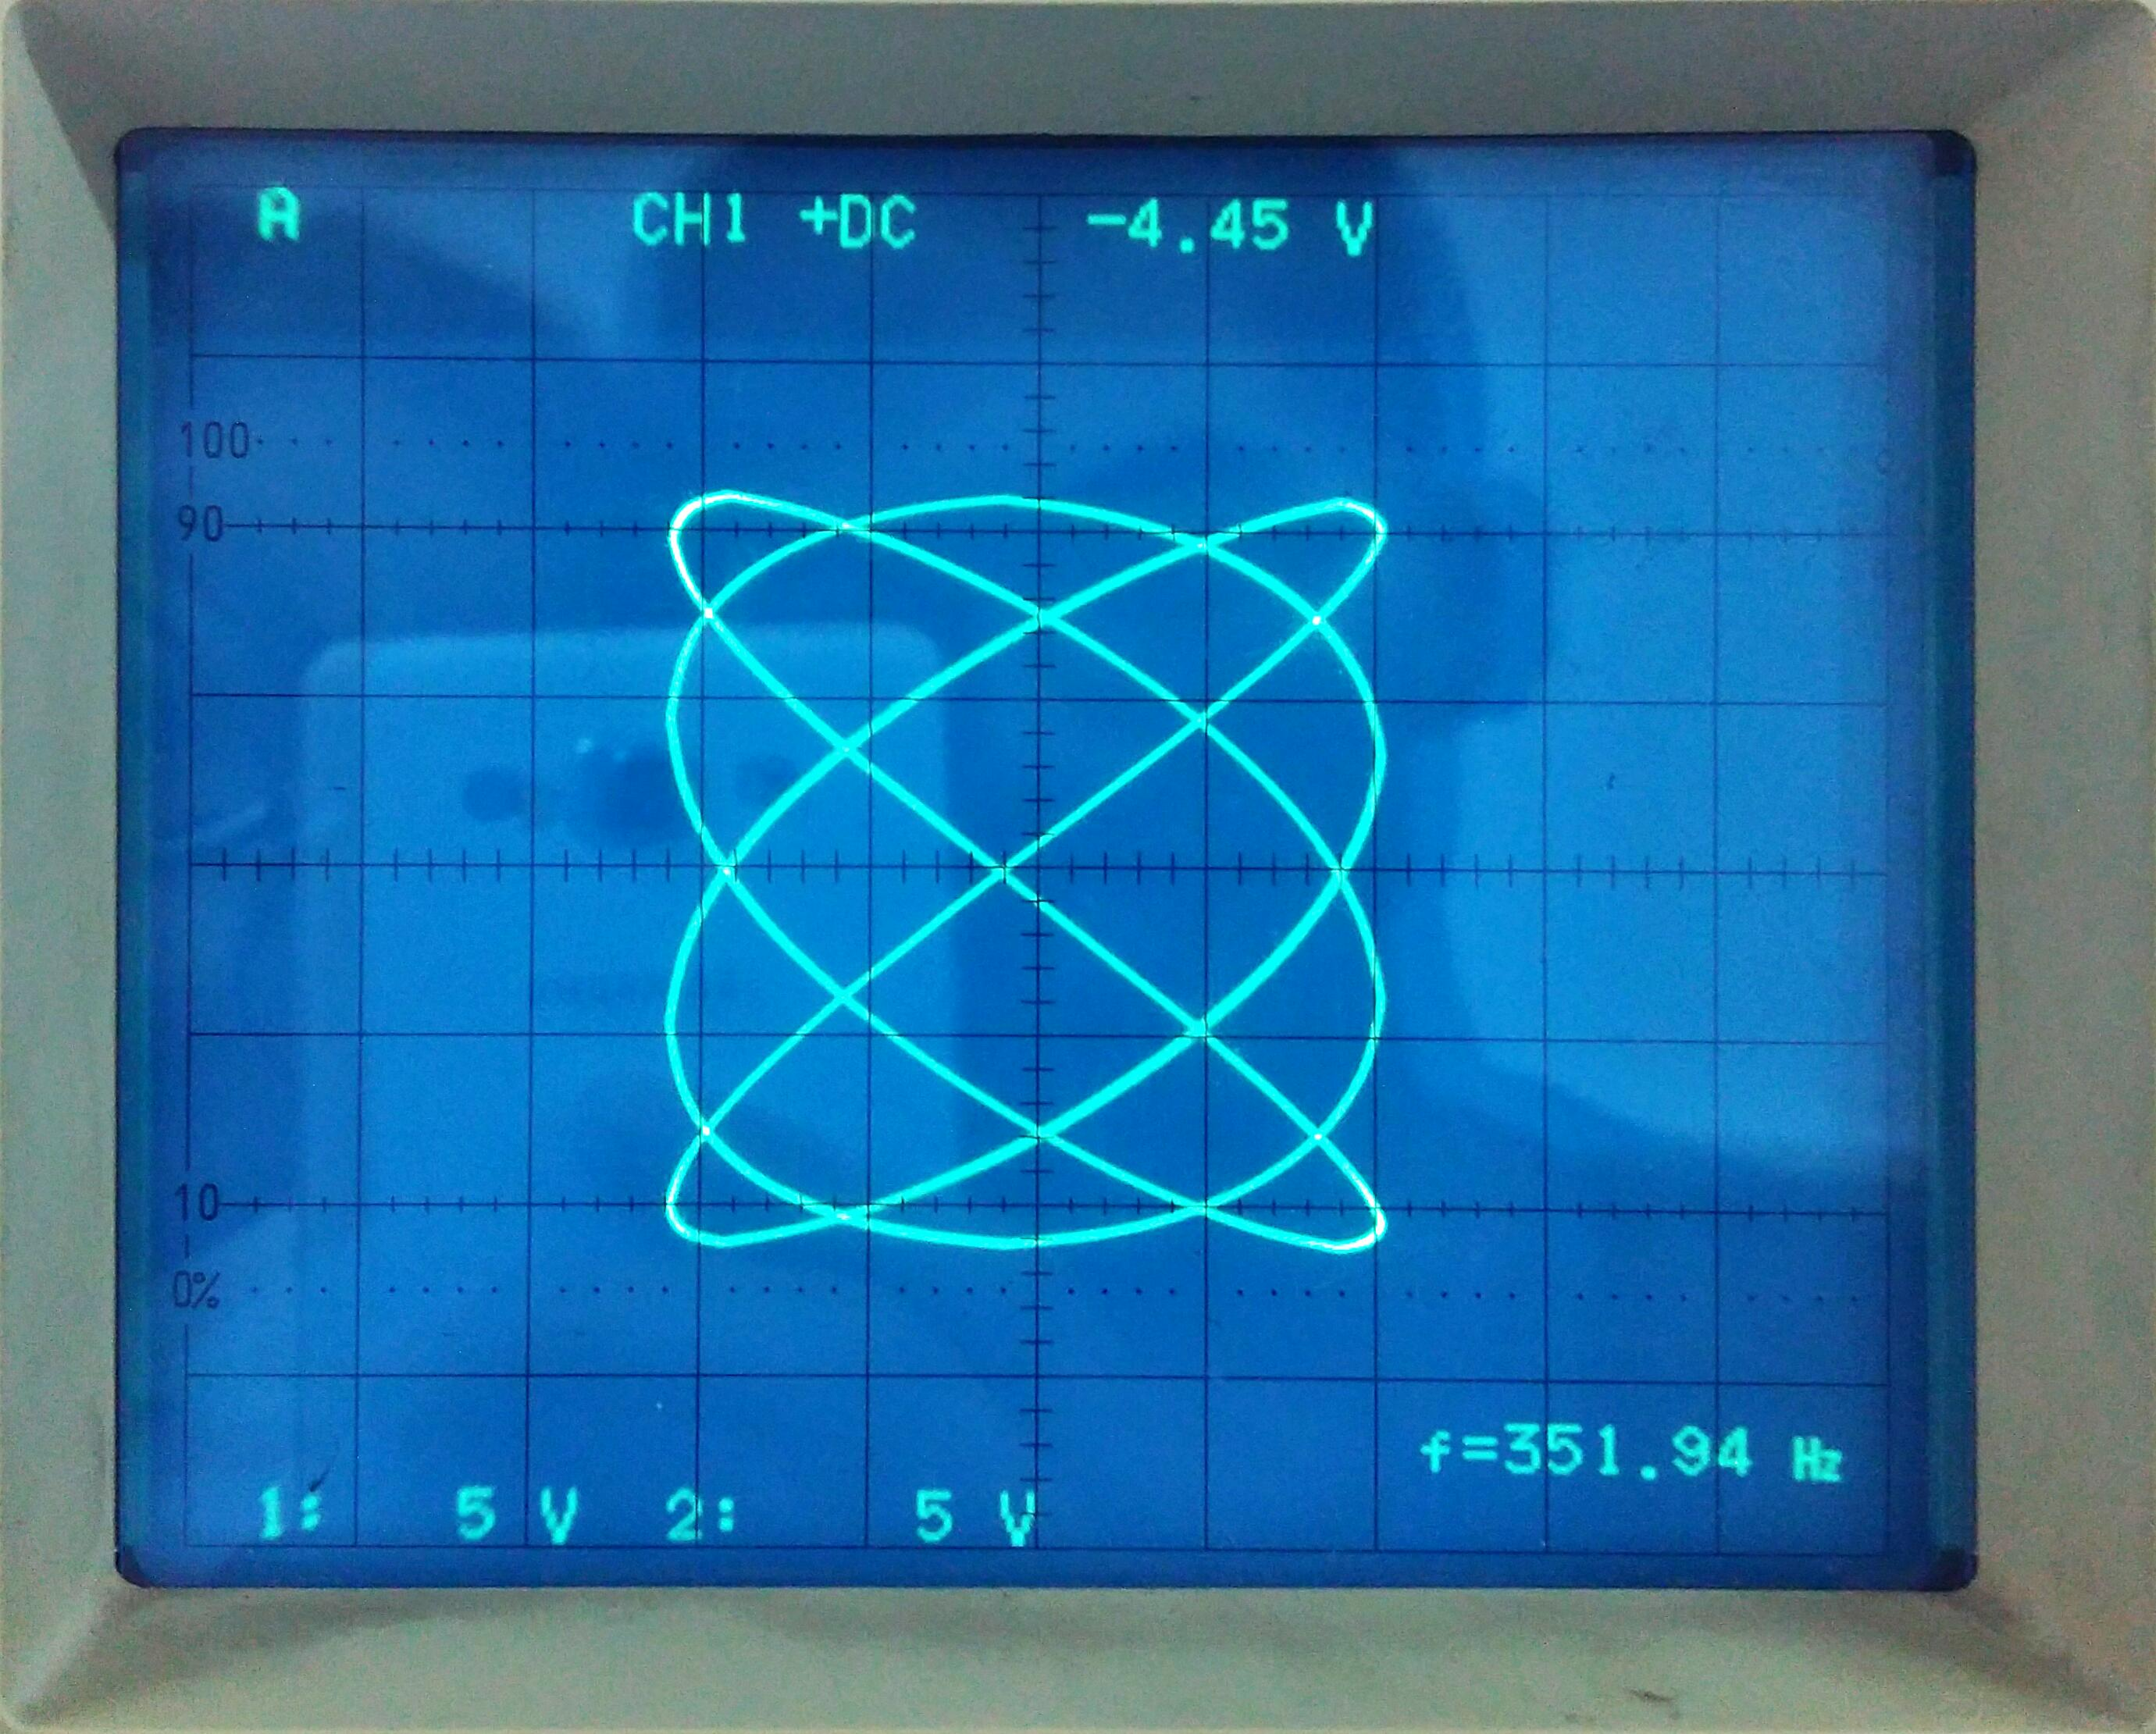
\includegraphics[scale=.1]{L09.jpg}
	\begin{center}
		\scriptsize Figure 9 利萨如图形9
	\end{center}

\end{figure}
	
\begin{figure}[htbp]
\centering

	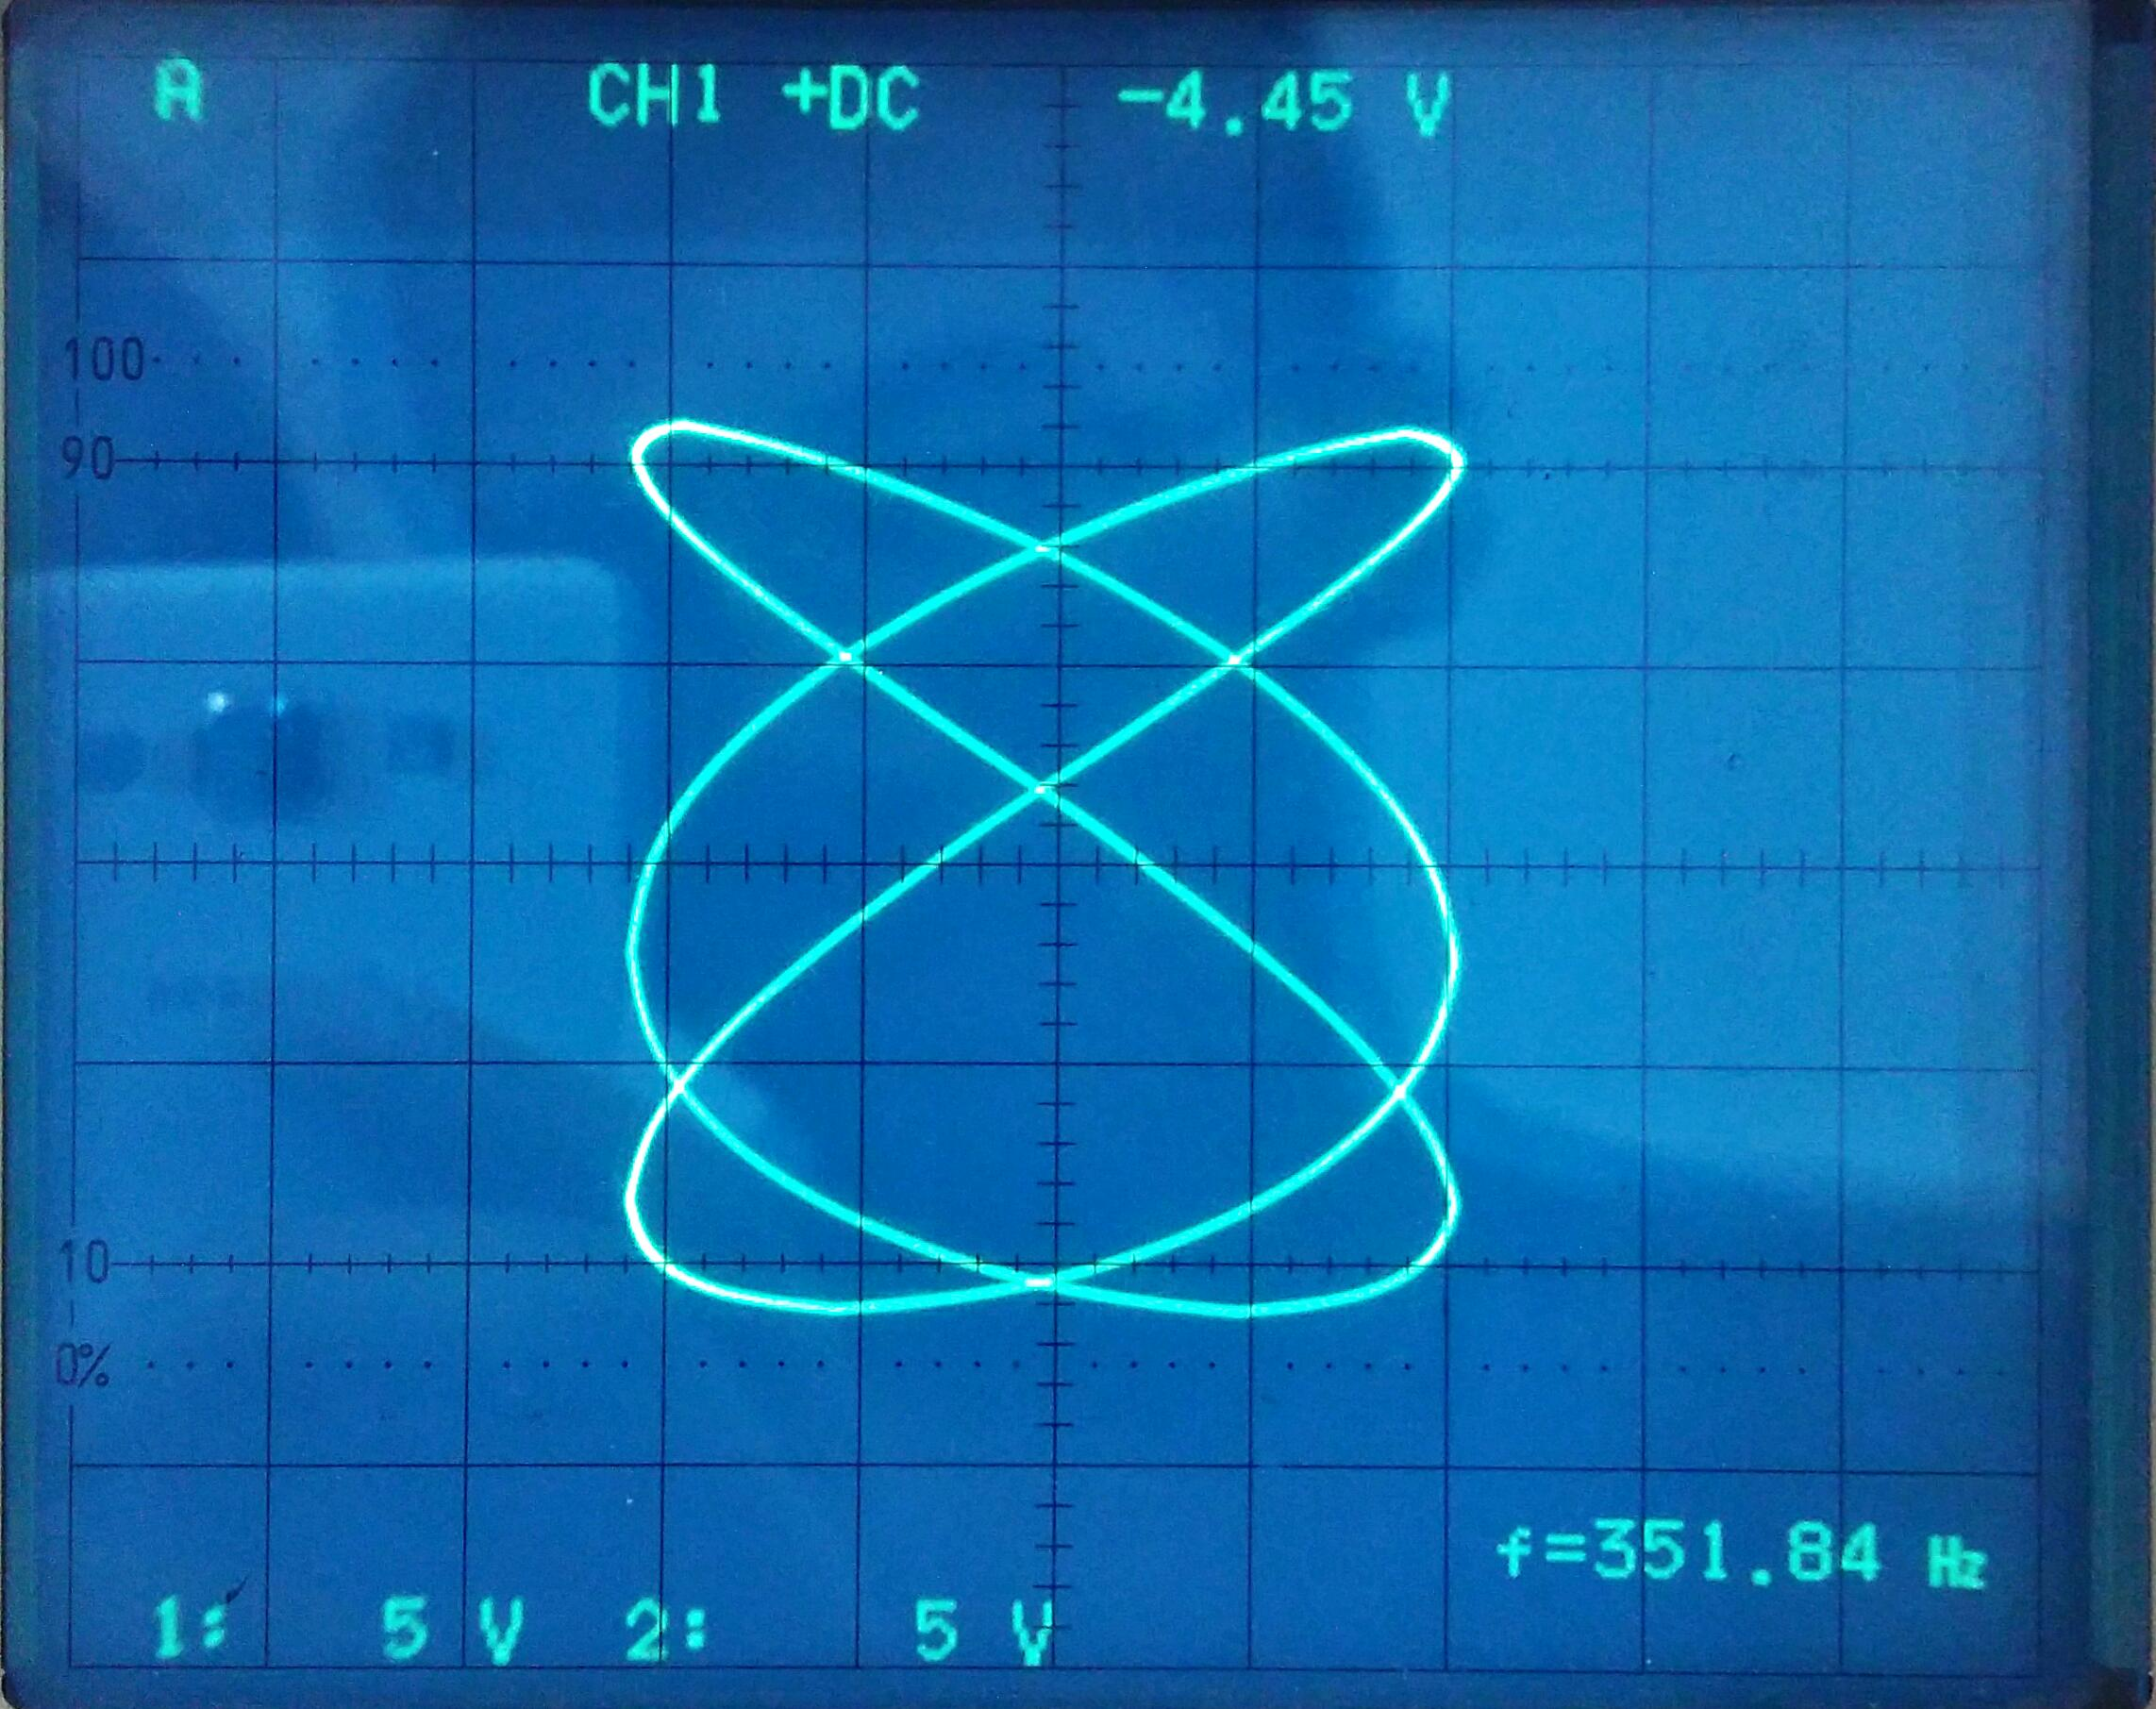
\includegraphics[scale=.11]{L10.jpg}
	\begin{center}
		\scriptsize Figure 10 利萨如图形10
	\end{center}

\end{figure}

\section*{二、分析和讨论}
\subsection*{1.测量仪器最小分度与测量结果有效数字的关系}
	
	示波器每一大格有5小格,我们应该在每一小格的精度基础上再估读一位.如果$t_0/5=2ms$,我们读到1ms即可,如果$K/5=1V$时,读到$0.1V$即可. \\
	
	如果涉及乘除运算,结果的有效数字应该向因数中最小的有效数字看齐.如果涉及加减,则应该向因数中末位最靠左的有效数字看齐. \\
	
\subsection*{2.利用利萨如图形计算信号的频率比和相位关系}

	两信号的频率比计算方法很简单.在垂直方向画一条直线,交图形于m个点;在水品方向也画一条线,交图形于n个点,则二者的频率比为: \\
	
\begin{equation}
	f_1 : f_2 = m : n
\end{equation}

	相位关系应分情况讨论.如果是同频振动的话,如果利萨如图形交x轴于$x_1$点,坐标轴长度为$x_0$,则 \\
	
\begin{equation}
	\Delta \phi = arcsin(\frac{x_1}{x_0})
\end{equation}

	如果二者频率不同,则它们没有稳定的相位差,不妨设初始时刻x方向相位恰好为0,有 \\
	
\begin{align}
	x = sin(n\omega_0 t) \\
	y = sin(m\omega_0 t + \phi) 
\end{align}

	为求得图形和y轴交点,不妨令$t=0$,我们有
	
\begin{equation}
	\phi = arcsin(\frac{y_1}{y_0}) + \frac{k\pi}{m}
\end{equation}

	上式中$\phi$有很多值可以取,这些值对应的都是同一种情况. \\
	
	为求得$x_0$与$y_0$,我们可以关掉一个信号发生器,这样屏幕上就只有一条直线,量取直线长度即可. \\
	
	不妨以图7为例,我们有:
	
\begin{align}
	f1 : f2 = 6 : 2 = 3 : 1 \\
	\phi \approx arcsin(\frac{0.5}{2.2}) + \frac{k\pi}{3} \approx 0.23  + \frac{k\pi}{3}
\end{align}
	
\section*{三、感悟和收获}

	示波器实验严格来说并不能算实验,只是帮助我们熟悉示波器这个仪器而已.但是操作过程中我还是遇到了很多问题,比如示波器被老师打乱之后确实花了不少时间手忙脚乱才调好.这告诉我:再简单的仪器,再简单的实验,都必须要认真对待! \\

\end{CJK*}
\end{document}
